%% THIS IS THE MAIN FILE %%
% Here the main arrangement of your thesis is determined. 
% In this file you read-in all chapters (as separate .tex files)
% This is also the file you 'Build' with a LaTeX editor, like TeXmaker.
% The .cls file (MScThesis.cls) contains all details regarding copyrights and so on. Take a look and adjust where applicable. But be careful changing this file: it determines the whole lay-out of your thesis!
% This MSc thesis standard layout is optimized for double sided printing on A4 format paper.
% Good luck and have fun with your Master Research in Applied Geophysics! Kind regards, Niels Grobbe

\documentclass[a4paper,11pt]{MScThesis}
%
%\usepackage{pifont}
\mscName{YourName}
\mscDate{\today}
\mscTitle{Test}
\mscSubTitle{Subtitle}
\mscKeyWords{thesis, msc, subject}
%
%\mscBackPicture{2660PF3}    % eps of 21 * 29.7 cm
\mscReaderOne{Name of first supervisor}
\mscReaderTwo{Name of second supervisor}
\mscReaderThree{Name of third supervisor or committee member}
%\mscReaderFour{}
%
\setThesisInfo
%
\begin{document}
%
%============================= Front matter ========================================
\frontmatter %
%
% Make a hell of a lot of title pages
    \maketitle
%
% Abstract
    \nonumchap{Abstract}

Please pay particular attention to the preparation of your abstract; use this text as a guide. Every master thesis report must be accompanied by an informative abstract of no more than one paragraph (max 300 words). The abstract should be self-contained. No references, figures, tables, or equations are allowed in an abstract. Do not use new terminology in an abstract unless it is defined or is well-known from the literature. The abstract must not simply list the topics covered in the paper but should (1) state the scope and principal objectives of the research, (2) describe the methods used, (3) summarize the results, and (4) state the principal conclusions. Do not refer to the master thesis report itself in the abstract. For example, do not say, "In this thesis we will discuss". Furthermore the abstract must stand alone as a very short version of the master thesis report rather than as a description of the contents. Remember that the abstract will be the first and most widely read portion of the master thesis report. Readers will be influenced by the abstract to the point that they decide to read the master thesis report or not.

    \cleardoublepage
%
% Acknowledgements
    \nonumchap{Acknowledgements}%
    First of all I want to thank all the people who have participated in this project ..
    Remember, often more people have (in some way) contributed to your final thesis than you would initially think of....
    \vspace*{15mm}

    \noindent
    Delft University of Technology \hfill \mscname\\ % choose the university where you carried out your final MSc thesis research
    Swiss Federal Institute of Technology \hfill \mscname\\ % choose the university where you carried out your final MSc thesis research
    RWTH Aachen University \hfill \mscname\\ % choose the university where you carried out your final MSc thesis research
    \mscdate

%
% table of contents, (\toc or \toclof or \tocloflot )
    \tocloflot
%
% Nomenclature
    \printnomencl %
%
% Acronyms
    \nonumchap{Acronyms} %
    %
    \begin{acronym}%
        \acro{DUT}{Delft University of Technology}%
        \acro{ETH}{Swiss Federal Institute of Technology}%
        \acro{RWTH}{Aachen University}%
    \end{acronym}%
    %
    \cleardoublepage%
%
%
%============================= Main matter =========================================
%
\mainmatter
%
% Introduction
\chapter{Introduction} \label{chap::intro}

    Welcome to the standard layout for your IDEA LEAGUE MSc thesis written in \LaTeX. \LaTeX\  has a variety of advantages over conventional/ standard text editing programs, which you will soon enough discover yourself. \LaTeX\  almost forms a standard in the Scientific Community, especially due to its effective and straightforward mathematical capabilities.\\
    This is Chapter\ \ref{chap::intro}. If you want to know more about \LaTeX\ you better read
    \cite{texbook} or use the extensive help available on the internet. \index{LaTeX}. This 'hidden' index command helps you making an index at the end of your thesis. You can add this flag anywhere you want to make an index hit. You can see here also how to use acronyms, like \ac{DUT}. The acronyms are automatically listed in the corresponding section. Also, hyperlinks are created automatically with the developed class file, such that your digital PDF version of your thesis can be read dynamically.
 Have fun with \LaTeX\ and your M.Sc. research project and good luck! \\ \\
 
The purpose of the introduction is to tell readers why they should want to read what follows the introduction. This chapter should provide sufficient background information to allow readers to understand the context and significance of the problem. This does not mean, however, that authors should use the introduction to rederive established results or to indulge in other needless repetition. The introduction should (1) present the nature and scope of the problem; (2) review the pertinent literature, within reason; (3) state the objectives; (4) describe the method of investigation; and (5) describe the principal results of the investigation. % notice how the reference to the introduction takes place.. It refers to the name.tex

\cleardoublepage

%
% First Part
    \part{First Part} % you can divide your thesis into different parts, for example Theory&Modeling in part 1 and real data examples in part 2.
		    \chapter{First Real Chapter}

    This is a demonstration chapter. I will explain some of the possibilities of \LaTeX. Here something will be shown of control theory, 'the transfer function' \lsymb{$H(s)$}{Transfer function}. Subscripts and superscripts can be put in the nomenclature \index{nomenclature} list. \supers{max}{Maximum} \subs{min}{Minimum} Other things can also be added to the nomenclature list, like explanations of symbols being used throughout the thesis. \others{[kts]}{Knots} \others{$^{\circ}$, [deg]}{Degrees}

        \section{First section}

        This is the section. Referring to equations, figures and tables can easily be done by the commands \verb"\eqnref{}",
        \verb"\figref{}" and \verb"\tabref{}".
        \begin{equation}\label{eq:First}
        H(s) = \frac{1}{s+2}
        \end{equation}

        You see? Refer to equations like this \eqnref{eq:First}, i.e. the name of the label you have given the specific equation, figure or table.
        
        \subsection{The first subsection}
  
        Now I demonstrate, numbering equations, using subequations:
	  \begin{subequations}
		\begin{eqnarray}
    \label{2eq1d1}
	  \nabla\times\mathbf{L}  &=& \frac{\partial\mathbf{G}}{\partial t} \\
    \label{2eq1d2}
  	\nabla\times\mathbf{G}  &=& \frac{\partial\mathbf{L}}{\partial t} + \mathbf{J} \\
    \label{2eq1d3}
    \mathbf{G}              &=& \sigma\mathbf{J}
		\end{eqnarray}
			  \end{subequations}
	
				Or we can make matrices:
				\begin{equation}
				\mathbf{Q}_{12}=\left[\begin{array}{ccc}
		          0  &     1          &  0 \\
	            1  &     0          &  1 \\
	            0  &     1          &  0 \\
       	\end{array}\right]\quad
        \nonumber
		    \label{2eq1cf}
		    \end{equation}
		    This can also be done using the \verb"\align{}" command. Equation arrays are also possible:
     		\begin{eqnarray}
    		\label{2eq1e1}
	  \nabla\times\mathbf{L}  &=& \frac{\partial\mathbf{G}}{\partial t} \\
	    	\label{2eq1e2}
  	\nabla\times\mathbf{G}  &=& \frac{\partial\mathbf{L}}{\partial t} + \mathbf{J} \\
		    \label{2eq1e3}
    \mathbf{G}              &=& \sigma\mathbf{J}
		  \end{eqnarray}

       
        \subsubsection[Subsection Short Title]{The first sub-subsection with a very very very long title, but in the table of contents one can only see the short title in square brackets}

                Impressed by the capabilities? \index{Nicecapabilities}
                If you want to know more about the capabilities of \LaTeX, take a look at the "\textbf{The Not So Short Introduction to \LaTeXe}", which can be found on the internet.

    \paragraph{Next paragraph.}
    \begin{figure}[htbp]  % fig 6.3 page 186 Turbulence and Remous
    \centering
    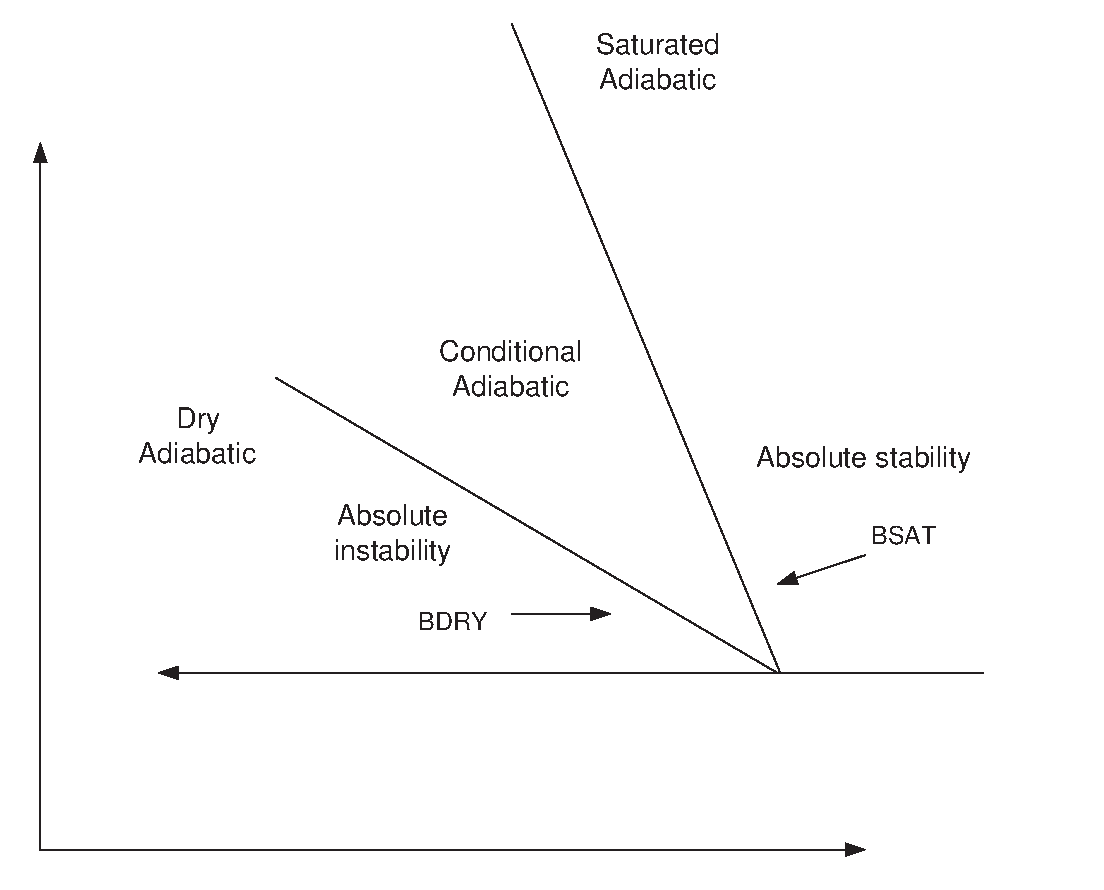
\includegraphics[width=11cm]{vertstab.eps}
    \caption{Stability conditions for the vertical stability of saturated and unsaturated air.} %this is how it shows up in the List of Figures
    \label{f:verticalstab}
    \end{figure}
.\\    
And finally I end this example file with a table which will be centered in the middle of the following page
\begin{table}[hp]
\centering
\renewcommand{\arraystretch}{1.5}
\begin{tabular}{|ll|}
\hline
\multicolumn{2}{|c|}{\bf\sffamily {\it Data} files listed in a table }\\
\hline\hline
\multicolumn{2}{|l|}{\bf\sffamily First part} \\
Fabracadabra.m	& - Saturation computation\\
Fobracadabra.m	& - Pressure computation\\
Fibricadibri.m	& - Permeability computation\\
&\\
\multicolumn{2}{|l|}{\bf\sffamily Structural rock model} \\
struct.m	& - Rock structural data using symmetric boundary condition \\
bstruct.m	& - Rock structural data using anti-symmetric boundary condition \\
\hline
\end{tabular}
\caption{Good-looking program data deck files.} %this is how it shows up in the List of Tables
\label{tbl:tbl}
\end{table}





%
% Bibliography
    \bibliographystyle{apalike}
    \printbib{MyBib} % in MyBib.bib you add all your reference information, following the correct format.
    % The *.bin file needs to be compiled using the Bib-compile option of your LaTeX text editor. Sometimes, the bib file needs to be built several times, as well as the main file, before all references occur correctly in your PDF.


%============================= Back matter =========================================
\appendix

    \chapter{The back of the thesis}

    \section{An appendix section}

    \subsection{An appendix subsection with C++ Lisitng}

    \lstset{language=C++}
    \lstinputlisting{test.c}

    \subsection{A \matlab $ $ Listing}

    \lstset{language=matlab}
    \lstinputlisting{test.m}

    \chapter{Yet another appendix}

    \section{Another test section}

    Ok, all is well.

% Index
    \printindex
    \cleardoublepage

\end{document}

